\section{eo\-Steady\-Fit\-Continue$<$ EOT $>$ Class Template Reference}
\label{classeo_steady_fit_continue}\index{eoSteadyFitContinue@{eoSteadyFitContinue}}
A continuator: does a minimum number of generations, then stops whenever a given number of generations takes place without improvement.  


{\tt \#include $<$eo\-Steady\-Fit\-Continue.h$>$}

Inheritance diagram for eo\-Steady\-Fit\-Continue$<$ EOT $>$::\begin{figure}[H]
\begin{center}
\leavevmode
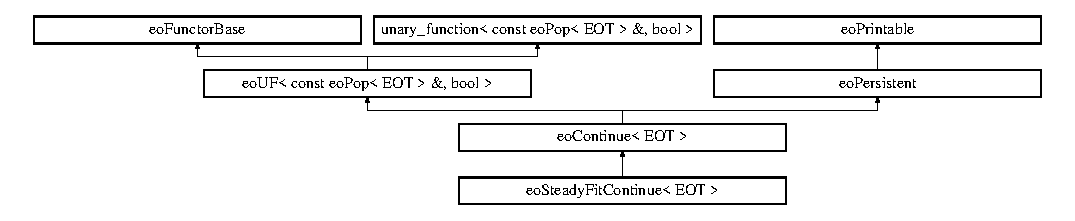
\includegraphics[height=2.52252cm]{classeo_steady_fit_continue}
\end{center}
\end{figure}
\subsection*{Public Types}
\begin{CompactItemize}
\item 
typedef EOT::Fitness {\bf Fitness}\label{classeo_steady_fit_continue_w0}

\end{CompactItemize}
\subsection*{Public Member Functions}
\begin{CompactItemize}
\item 
{\bf eo\-Steady\-Fit\-Continue} (unsigned long \_\-min\-Gens, unsigned long \_\-steady\-Gens)\label{classeo_steady_fit_continue_a0}

\begin{CompactList}\small\item\em Ctor for setting a. \item\end{CompactList}\item 
{\bf eo\-Steady\-Fit\-Continue} (unsigned long \_\-min\-Gens, unsigned long \_\-steady\-Gen, unsigned long \&\_\-current\-Gen)\label{classeo_steady_fit_continue_a1}

\begin{CompactList}\small\item\em Ctor for enabling the save/load the no. of generations counted. \item\end{CompactList}\item 
virtual bool {\bf operator()} (const {\bf eo\-Pop}$<$ {\bf EOT} $>$ \&\_\-v\-EO)\label{classeo_steady_fit_continue_a2}

\begin{CompactList}\small\item\em Returns false when a certain number of generations is reached withtout improvement. \item\end{CompactList}\item 
virtual void {\bf total\-Generations} (unsigned long \_\-mg, unsigned long \_\-sg)
\begin{CompactList}\small\item\em Sets the parameters (minimum nb of gen. \item\end{CompactList}\item 
virtual void {\bf reset} ()\label{classeo_steady_fit_continue_a4}

\begin{CompactList}\small\item\em Resets the state after it's been reached. \item\end{CompactList}\item 
virtual unsigned long {\bf min\-Generations} ()\label{classeo_steady_fit_continue_a5}

\begin{CompactList}\small\item\em accessors \item\end{CompactList}\item 
virtual unsigned long {\bf steady\-Generations} ()\label{classeo_steady_fit_continue_a6}

\item 
virtual std::string {\bf class\-Name} (void) const \label{classeo_steady_fit_continue_a7}

\end{CompactItemize}
\subsection*{Private Attributes}
\begin{CompactItemize}
\item 
unsigned long {\bf rep\-Min\-Generations}\label{classeo_steady_fit_continue_r0}

\item 
unsigned long {\bf rep\-Steady\-Generations}\label{classeo_steady_fit_continue_r1}

\item 
bool {\bf steady\-State}\label{classeo_steady_fit_continue_r2}

\item 
unsigned long {\bf this\-Generation\-Place\-Holder}\label{classeo_steady_fit_continue_r3}

\item 
unsigned long \& {\bf this\-Generation}\label{classeo_steady_fit_continue_r4}

\item 
unsigned int {\bf last\-Improvement}\label{classeo_steady_fit_continue_r5}

\item 
Fitness {\bf best\-So\-Far}\label{classeo_steady_fit_continue_r6}

\end{CompactItemize}


\subsection{Detailed Description}
\subsubsection*{template$<$class EOT$>$ class eo\-Steady\-Fit\-Continue$<$ EOT $>$}

A continuator: does a minimum number of generations, then stops whenever a given number of generations takes place without improvement. 



Definition at line 35 of file eo\-Steady\-Fit\-Continue.h.

\subsection{Member Function Documentation}
\index{eoSteadyFitContinue@{eo\-Steady\-Fit\-Continue}!totalGenerations@{totalGenerations}}
\index{totalGenerations@{totalGenerations}!eoSteadyFitContinue@{eo\-Steady\-Fit\-Continue}}
\subsubsection{\setlength{\rightskip}{0pt plus 5cm}template$<$class EOT$>$ virtual void {\bf eo\-Steady\-Fit\-Continue}$<$ {\bf EOT} $>$::total\-Generations (unsigned long {\em \_\-mg}, unsigned long {\em \_\-sg})\hspace{0.3cm}{\tt  [inline, virtual]}}\label{classeo_steady_fit_continue_a3}


Sets the parameters (minimum nb of gen. 

+ steady nb of gen.) and sets the current generation to 0 (the begin) 

Definition at line 84 of file eo\-Steady\-Fit\-Continue.h.

References eo\-Steady\-Fit\-Continue$<$ EOT $>$::reset().

The documentation for this class was generated from the following file:\begin{CompactItemize}
\item 
eo\-Steady\-Fit\-Continue.h\end{CompactItemize}
